%designed for PDFLaTeX
\documentclass[]{beamer}
\usetheme{Antibes}%{Frankfurt}%{Berlin}%{Boadilla}

\usepackage[utf8]{inputenc}
\usepackage[english]{babel}
\usepackage{graphicx}
\usepackage{upquote}
\usepackage{listings}
\usepackage{verbatim}
\usepackage{multicol}

\setlength{\parskip}{\medskipamount}
\setlength{\parindent}{0pt}

\title{Comparative Study of Intrinsic Metrics on 3D-Shapes}
\author{Frank Schmidt}
\institute{Computer Vision Group - Technische Universit\"{a}t M\"{u}nchen}
\date{31.10.2014}

%\setbeamertemplate{note page}[plain] %need less gray ink for printing
\setbeameroption{show notes} %comment this for a version without notes

\begin{document}

	\begin{frame}
		\titlepage
	\end{frame}

	\begin{frame}
		\tableofcontents
	\end{frame}

	\begin{frame}
		some stuff about why this is important\\
		picture of 3d-model with different paths as minimal?
	\end{frame}

\section{Background Theory}
\subsection{Shapes as Metric Spaces}
	\begin{frame}
		Metric Space\\
		A set $M$ and a metric function $d_M: M \times M \rightarrow R_+ \cup \{0,\infty\}$ are a metric space, iff for all $x,y\in M$:
		\begin{itemize}
			\item $d_M(x,y) = 0 \Leftrightarrow x = y$ (identity of indiscernibles)
			\item $d_M(x,y) = d_M(y,x)$ (symmetry)
			\item $d_M(x,y) \le d_M(x,z) + d_M(z,y)\,\forall x,y,z \in M$ (triangle inequality)
		\end{itemize}
		\note{isometry: distance preserving, surjective map; $d_X(x,y) = d_Y(f(x),f(y))$}
		\note{compact metric space: closed/ complete and totally bounded; reasonable since we approx. by meshes}
		\note{resticting ambient space metric to set possible; intrinsic metrics might be simpler}
	\end{frame}

	\begin{frame}
		Hausdorff Distance\\
		\includegraphics[width=\textwidth]{t_pictures/hausdorff} \\

		Gromov-Hausdorff Distance
		$$d_{GH}(X,Y) = \inf_{Z,f,g} d^Z_{GH} (f(X),g(Y))$$
		$$d_{GH}(X,Y) = \frac{1}{2} \inf_{R \subset X \times Y} dis \, R$$

		\note{need means to define closeness of surfaces; regular surface simpler with surface patches, small differences mean small distance}
		\note{H distance: $d^Z_H = max(sup_X(d_Z(x,Y)),sup_Y(d_Z(y,X)))$ having same ambient space}
		\note{GH distance: use isometric embeddings to embed shapes in common metric space; select the 'best' one}
		\note{reduce computation effort for GH: use correspondences with notion of distortion (biggest metric change between two points) and r-coverings/FPS (since it is consistent to sampling)}
	\end{frame}

\subsection{Differential Geometry}
	\begin{frame}
		\note{regular surfaces approximated by piecewise linear triangular meshes, restricting to those without boundary (no extra conditions)}
		\includegraphics[width=0.8\textwidth]{t_pictures/regular_surface}\\
		Regular Surfaces/ First Fundamental form\\
		$$I_p(w) =  \langle w,w\rangle_p = |w|^2 > 0; I_p(w) = \begin{pmatrix} u' & v' \end{pmatrix} \begin{pmatrix} E & F \\ F & G \end{pmatrix} \begin{pmatrix}u' \\ v'\end{pmatrix}$$
		\note{reg surface: a set of $R^3$ with a map x from $R^2$ with 1.x differentiable 2.x homeomorphism (has $x^{-1}$) 3. differential $dx_q: R^2 \rightarrow R^3$ has full rank}
		\note{1."differential" geometry 2. no self intersections 3. tangent planes are not degenerated}
		\note{differential: maps tangential vectors to tangential vectors}
		\note{independent of parametrisation (go in a triangle from one parameter domain to the other)}
		\note{functions on surfaces: use map $x^{-1}$ to calculate them in the parameter domain}
		\note{tangent plane and differential (2x3 array, differentiated by uv of the different elements of x)}
		\note{FFF: ``natural inner product on the surface'', invariant to isometries, matrix is result of $dx_q * dx_q^T$, therefore differential has to have full rank so that
			  the resulting tangent plane is not one dimensional}
	\end{frame}

	\begin{frame}
		Laplace-Beltrami operator: equivalent to the Laplace operator in Euclidean space
		$$\Delta f = div (\nabla f)$$
		$\Delta f$ is linear $\Rightarrow \Delta f$ has to have eigenfunctions fulfilling $\Delta f = \lambda f$
		\note{Discretization: using Finite Elements and the cotan-method to obtain $M^{-1}Cf = Lf$ with M dependent on the triangle areas and C dependent on the angles}
		\note{Basic idea: $f = \sum f_i \phi_i$ with coefficients $f_i$ and basic functions $\phi_i$ (e.g. hat function at vertex i)}
		\note{function f = values of the function at all vertices, linear interpolation between them}
		\note{LB operator is linear, since we can represent it as a matrix}
		\note{Laplacian eigenfunctions: somewhat similar to Fourier transformation, different frequencies of a function}
		\note{in case of head diffusion: heat operator (heat distro after time $t$) and LB operator map from S to S, and are related by $H_t = e^{-\lambda \Delta_S}$, hence
			  same eigenfunctions, scaled eigenfunctions}
	\end{frame}
% Regular Surfaces, Laplace-Beltrami operator

\section{Intrinsic Metrics}
	\begin{frame}
		%TODO
		euclidean distance? Show example (not intrinsic)
	\end{frame}

\subsection{Geodesic Distance}
	\begin{frame}
		Geodesic Distance: length of the shortest path on the surface between two points
		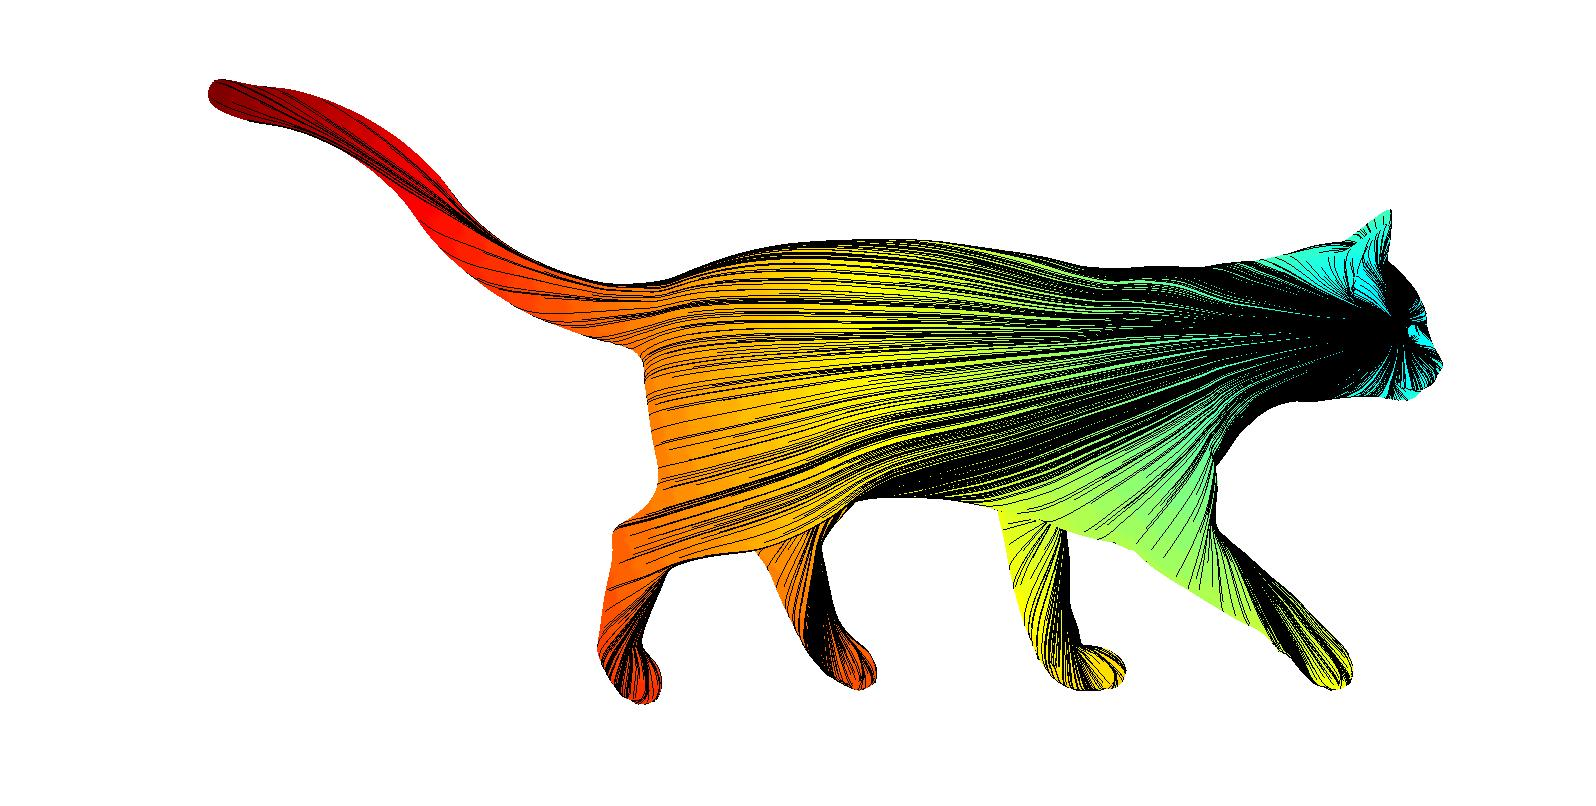
\includegraphics[width=0.8\textwidth]{t_pictures/cat_geodesic_paths}\\
		\note{note sure how much to tell here \ldots basic idea is to define a ``straight'' line between two points}
		\note{keywords: regular, parametrized curve, where the covariant derivative of its tangent vectors (projection of the (tangent) vectors derivative to the tangent plane)
			  is zero (called parallel vector field).}
		\note{intrinsic, since only dependent on covariant derivative, which can be expressed in Christoffel symbols, which are only dependent on the FFF}
		\note{for the existence of shortest geodesics, the surface has to be complete, otherwise there is the hole-example}
		\note{geodesic stuff, telling you that the geodesic is only dependent on the
			first fundamental form; shortest straight distance on the surface\\
			Perhaps another slide to show stuff about the implementation?}
	\end{frame}

	\begin{frame}
		Discretisation to triangulated meshes:
		\begin{enumerate}
			\item geodesics need to be straight lines within each face
			\item when crossing an edge, the geodesic has to correspond to a straight line if the adjacent faces are unfolded into a common plane
			\item Combine multiple geodesics into a single data structure called window, which are propagated over the whole mesh in a Dijkstra like fashion
		\end{enumerate}
		\includegraphics[width=\textwidth]{t_pictures/geodesics_new_windows} \\
		\note{alternative implementation: solving the eikonal equation using the fast marching method}
		\note{window parameters, propagation, intersection; resulting in windows that can be used to backtrack the geodesic distance}
		\note{special treatment of saddle/boundary vertices}
	\end{frame}

\subsection{Diffusion Distance}
	\begin{frame}
		Diffusion Distance: measures the amount of heat transfered between two points after a certain time interval \\
		tradeoff between local and global properties depending on the time parameter
		%TODO heat equation/ heat kernel/computation equation
		%depends on time steps (2 pics) for local/global preference
%%%%%%%%%%%%%%%%%%%%%%%%%%%%%%%%%%%%%%%%%%%%%%%		\includegraphics[width=0.45\textwidth]{shrec2010_0001.topology.2_2.tiff}
%%%%%%%%%%%%%%%%%%%%%%%%%%%%%%%%%%%%%%%%%%%%%%%		\includegraphics[width=0.45\textwidth]{shrec2010_0001.topology.2_3.tiff}

	\end{frame}

\subsection{Commute-Time Distance}
	\begin{frame}
		Commute-Time Distance: Integral of the Diffusion Distance over all time steps
		%TODO more stuff here, otherwise it is so empty/ vllt equations from diffusion + commute time
		\note{tries to combine local and global properties}
	\end{frame}

\subsection{Biharmonic Distance}
	\begin{frame}
		(Almost) latest invention, tries to combine local and global properties;\\
		Also a pic would be nice probably
	\end{frame}

\section{Testing and Implementation}
\subsection*{}
	\begin{frame}
		3 tests: speed, visually compare plots under different changes of the mesh
		and an error analysis using one to one correspondances\\
		oh, and Farthest point sampling
	\end{frame}

	\begin{frame}
		some implementation stuff i find, otherwise this slide will be not existant
	\end{frame}

\section{Results}
\subsection*{}
	\begin{frame}
		a bunch of pictures of the different metrics, tables and stuff\\
		overall the biharmonic distance is the best
	\end{frame}
%each for itself/together; watch, if my graphics are applicable or need to be made smaller

%conclusion: it was great i did that, because ...

	\begin{frame}
		\centering \large
		Thank you for your attention.\\
		Any Questions?
	\end{frame}

\section*{} %%appendix
\appendix
	\begin{frame}{Sources}
		stuff
	\end{frame}

\end{document}
